% ---------------------------- Preamble starts here ----------------------------

\documentclass{beamer}

% --- Set beamer theme
\usetheme{Boadilla}
\setbeamertemplate{footline}{}				% Remove automatic footer
\setbeamertemplate{navigation symbols}{}	% Comment this line to display navigation symbols

% Load i2i symbol 
\addtobeamertemplate{frametitle}{}{%
\begin{textblock*}{\linewidth}(0cm,8cm)
		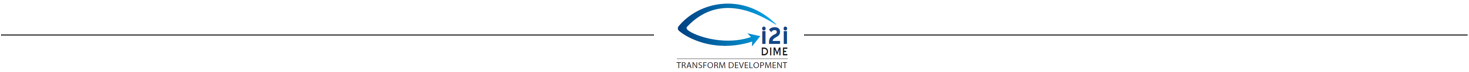
\includegraphics[width=\linewidth]{img/Footer.png}
\end{textblock*}}

% --- Load packages
\usepackage{textpos}		% To align objects correctly
\usepackage{multicol}		% To right in multiple columns
\usepackage{color}			% To color text

% --- Add your information here
\title{DIME Beamer Template}
\author{Add your name here}
\institute{DIME - World Bank}
\date{\today}

% ---------------------------- Preamble ends here ----------------------------

\begin{document}
	
\begin{frame}
	
\includegraphics[width=\textwidth]{img/Header.png}
	\vspace{-0.2cm}
	\titlepage 	 % Opening slide, prints inform
\end{frame}

\begin{frame}
\frametitle{Overview} % Table of contents slide, comment this block out to remove it
\tableofcontents % Throughout your presentation, if you choose to use \section{} and \subsection{} commands, these will automatically be printed on this slide as an overview of your presentation
\end{frame}

\section{Text}
\subsection{Simple text}

\begin{frame}
\frametitle{Paragraphs of Text}
Sed iaculis dapibus gravida. Morbi sed tortor erat, nec interdum arcu. Sed id lorem lectus. Quisque viverra augue id sem ornare non aliquam nibh tristique. Aenean in ligula nisl. Nulla sed tellus ipsum. Donec vestibulum ligula non lorem vulputate fermentum accumsan neque mollis.\\~\\

Sed diam enim, sagittis nec condimentum sit amet, ullamcorper sit amet libero. Aliquam vel dui orci, a porta odio. Nullam id suscipit ipsum. Aenean lobortis commodo sem, ut commodo leo gravida vitae. Pellentesque vehicula ante iaculis arcu pretium rutrum eget sit amet purus. Integer ornare nulla quis neque ultrices lobortis. Vestibulum ultrices tincidunt libero, quis commodo erat ullamcorper id.
\end{frame}

\subsection{Highlighted text}
\begin{frame}
\frametitle{Blocks of Highlighted Text}
\begin{block}{Title}
	Lorem ipsum dolor sit amet, consectetur adipiscing elit. Integer lectus nisl, ultricies in feugiat rutrum, porttitor sit amet augue. Aliquam ut tortor mauris. Sed volutpat ante purus, quis accumsan dolor.
\end{block}


\end{frame}

\subsection{Columns}
\begin{frame}
\frametitle{Multiple Columns}
\begin{columns}[c] % The "c" option specifies centered vertical alignment while the "t" option is used for top vertical alignment
	
	\column{.45\textwidth} % Left column and width
	\textbf{Heading}
	\begin{enumerate}
		\item Statement
		\item Explanation
		\item Example
	\end{enumerate}
	
	\column{.5\textwidth} % Right column and width
	Lorem ipsum dolor sit amet, consectetur adipiscing elit. Integer lectus nisl, ultricies in feugiat rutrum, porttitor sit amet augue. Aliquam ut tortor mauris. Sed volutpat ante purus, quis accumsan dolor.
	
\end{columns}
\end{frame}

\subsection{Items}
\begin{frame}{Add items}	

\begin{itemize}
	\item Currently, a lot of us, export tables from Stata and then copy paste the tables on to Excel and then to Word or something similar. 
	\item {\LaTeX} allows us to create a document once and every time a do-file is run, the tables are automatically updated in our {\LaTeX} document.
	\item This saves us a lot of time in the long run even though the learning curve for {\LaTeX} is a bit complicated compared to MS Word. 
	
\end{itemize}
\end{frame}

\begin{frame}{Add items sequentially}	

	\begin{itemize}
		\item<1->Currently, a lot of us, export tables from Stata and then copy paste the tables on to Excel and then to Word or something similar. 
		\item<2->{\LaTeX} allows us to create a document once and every time a do-file is run, the tables are automatically updated in our {\LaTeX} document.
		\item<3->This saves us a lot of time in the long run even though the learning curve for {\LaTeX} is a bit complicated compared to MS Word. 
		
	\end{itemize}
\end{frame}

\section{Images}
\begin{frame}{Add image}	

	\begin{figure}
		\centering
		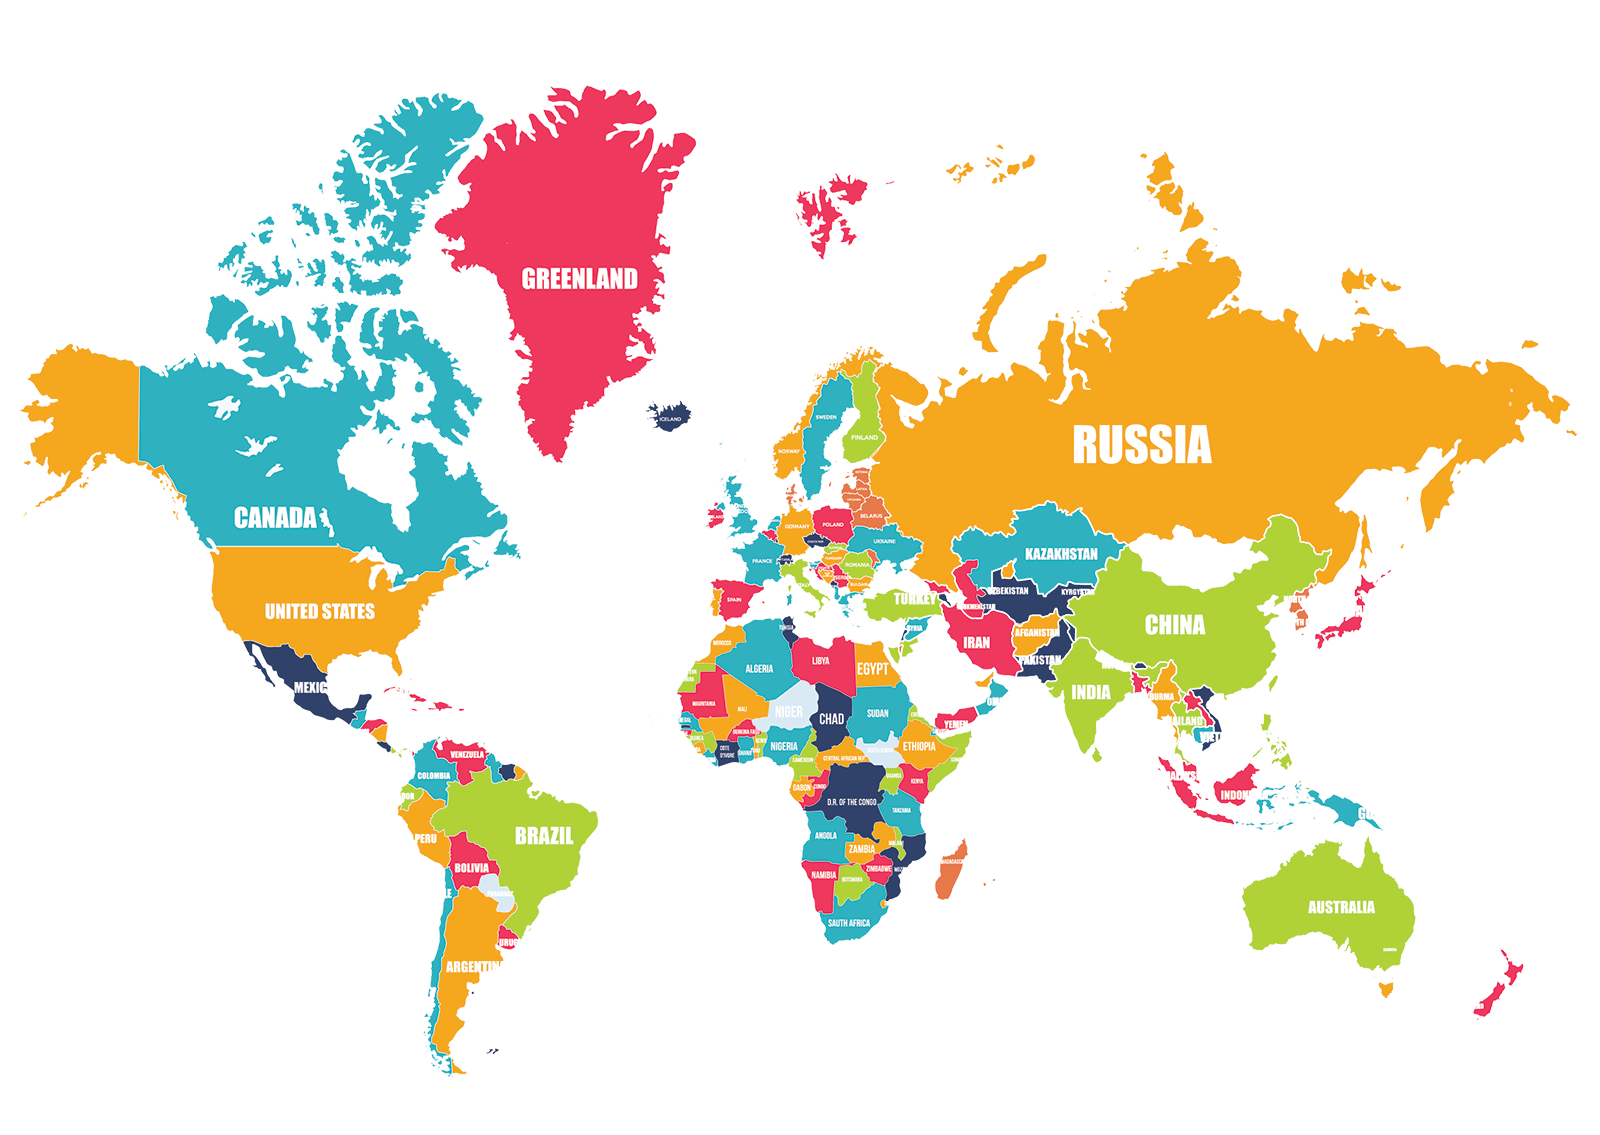
\includegraphics[height=.7\textheight]{img/world-map}
		\caption{World map}
		\label{fig:world-map}
	\end{figure}
	
\end{frame}

\begin{frame}{Add more than one image}

You can also display two images side by side

	\begin{multicols}{2}
		
		\begin{figure}
			\centering
			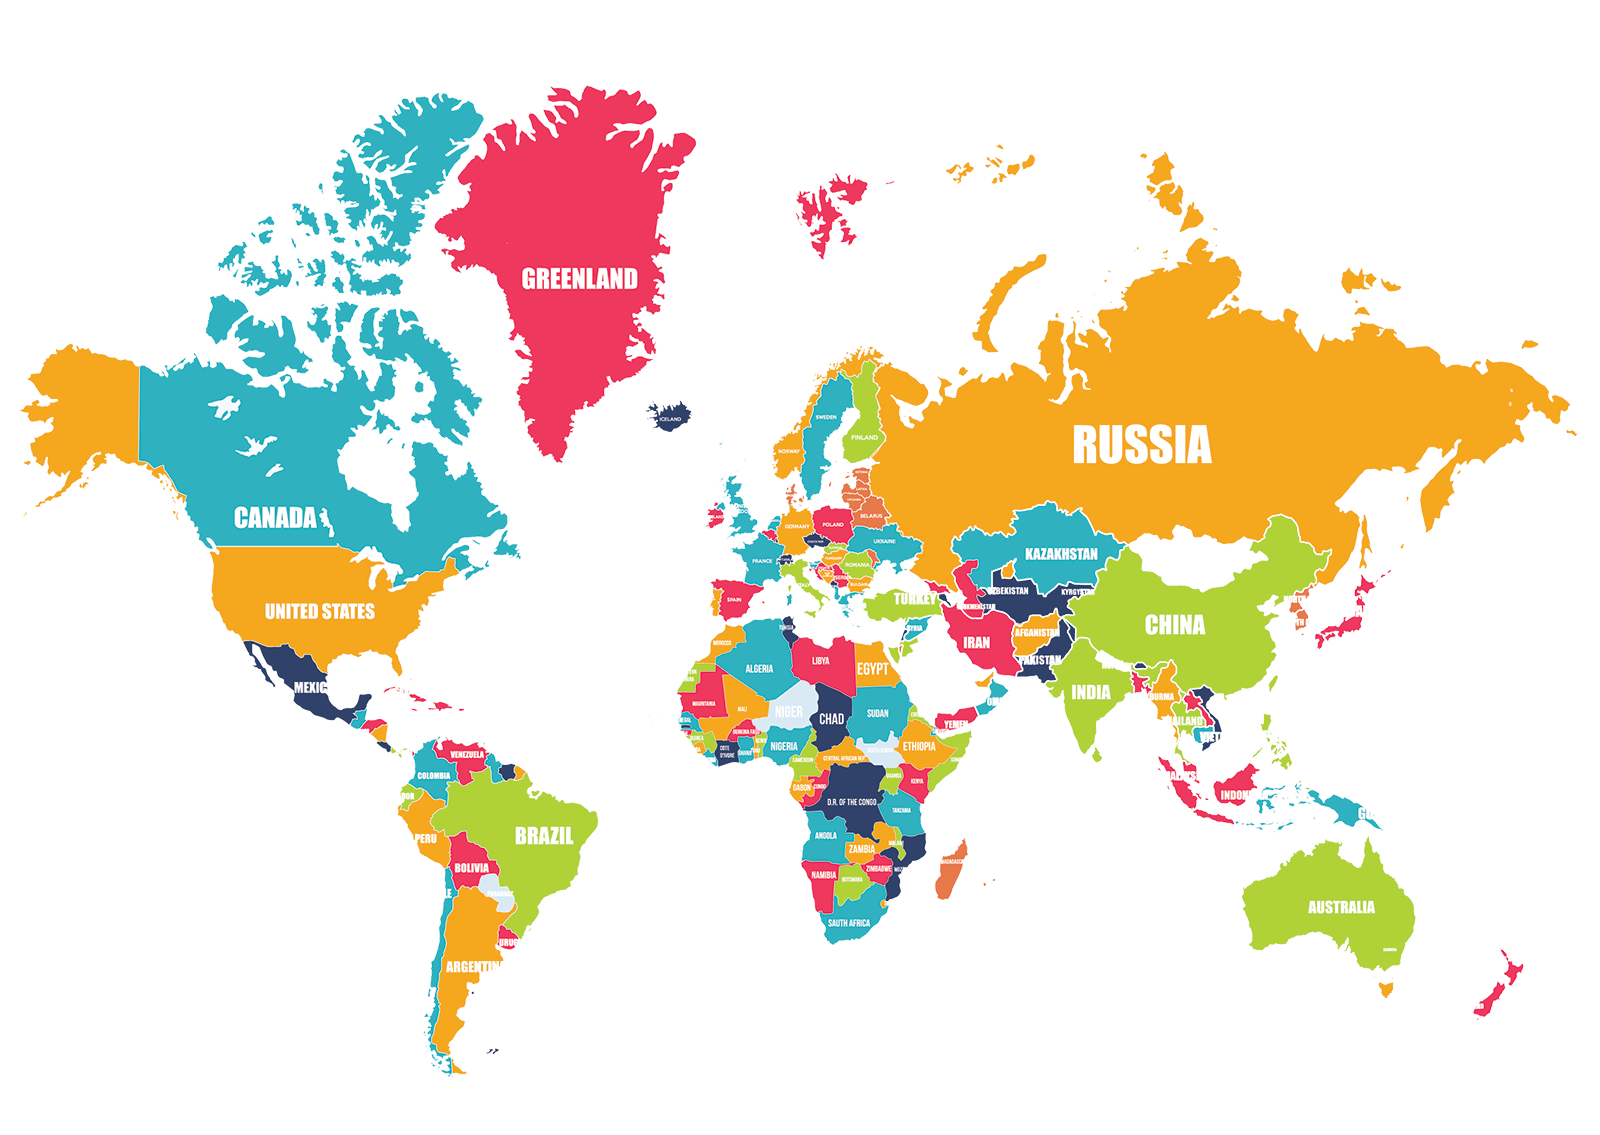
\includegraphics[width=\linewidth]{img/world-map}
			\caption{World map 1}
			\label{fig:world-map1}
		\end{figure}
		\begin{figure}
			\centering
			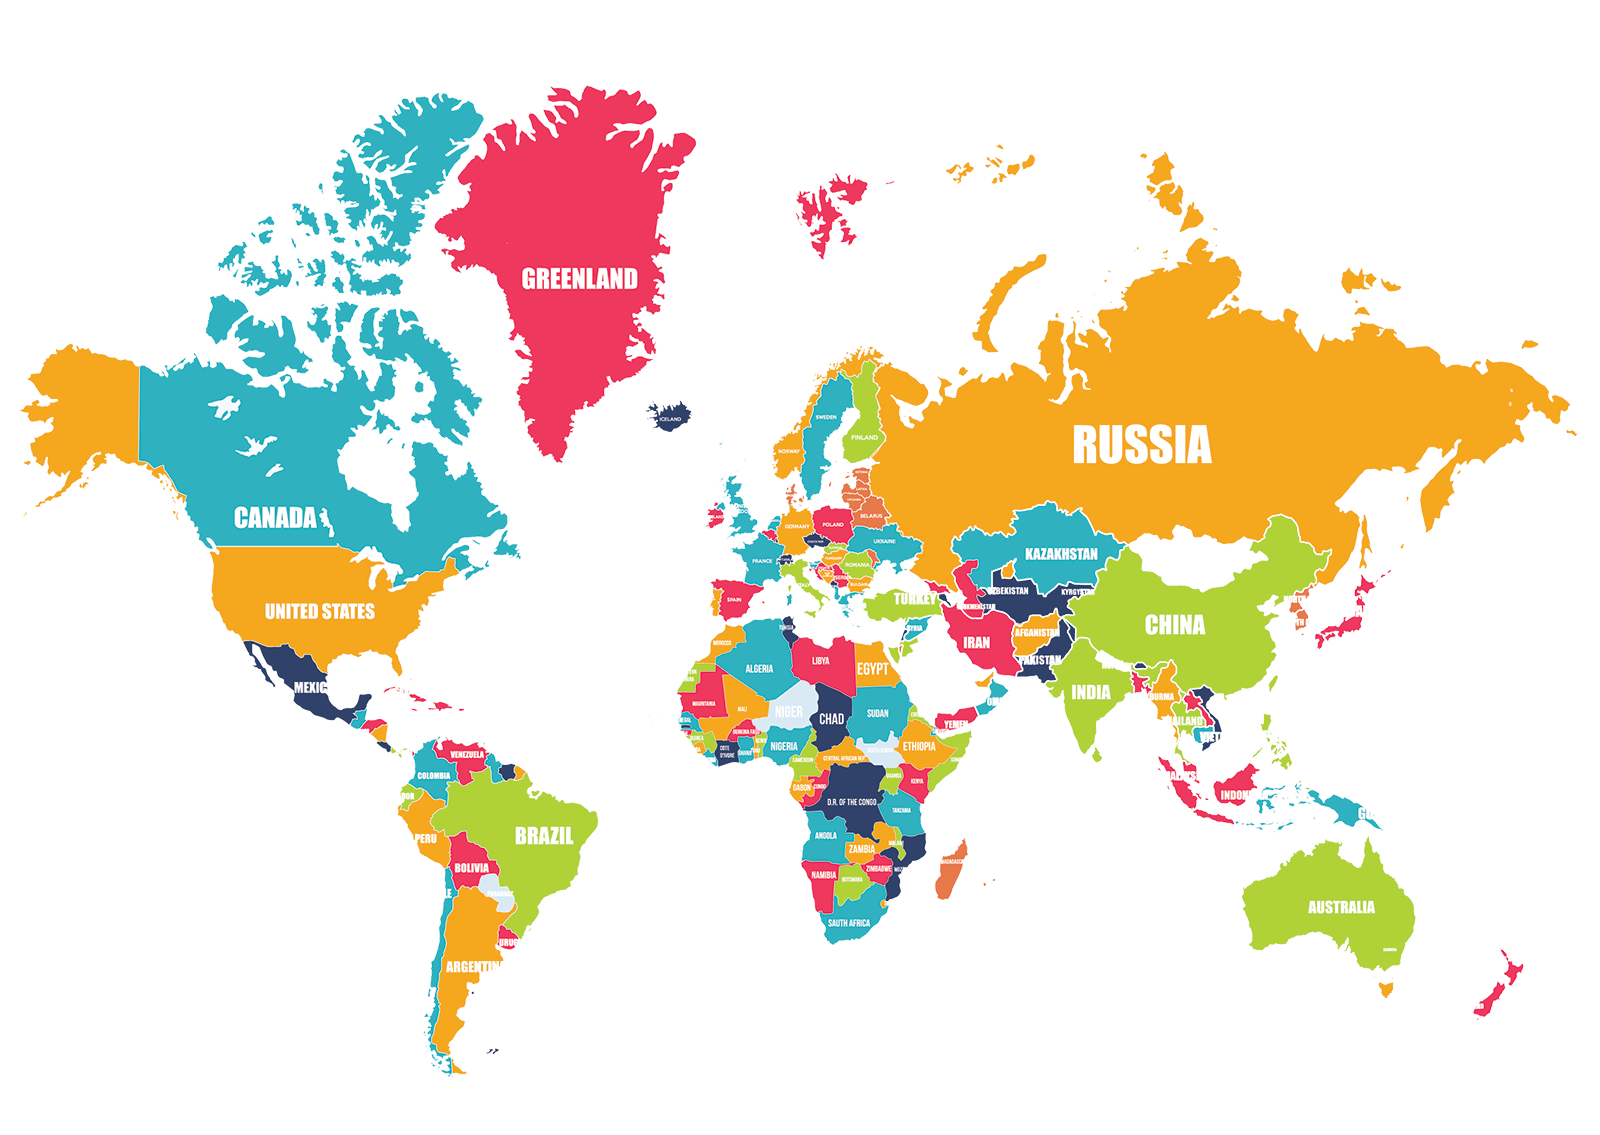
\includegraphics[width=\linewidth]{img/world-map}
			\caption{World map 2}
			\label{fig:world-map2}
		\end{figure}
	
	\end{multicols}

\end{frame}

\begin{frame}{Add image and text}

Lorem ipsum dolor sit amet, consectetur adipiscing elit

	\begin{multicols}{2}
		
		\begin{itemize}
			\item Mauris ut justo aliquam, consequat diam vitae, hendrerit felis
			\item Suspendisse ullamcorper tincidunt posuere
			\item Quisque vitae ipsum in massa commodo mattis
		\end{itemize}
		\begin{figure}
			\centering
			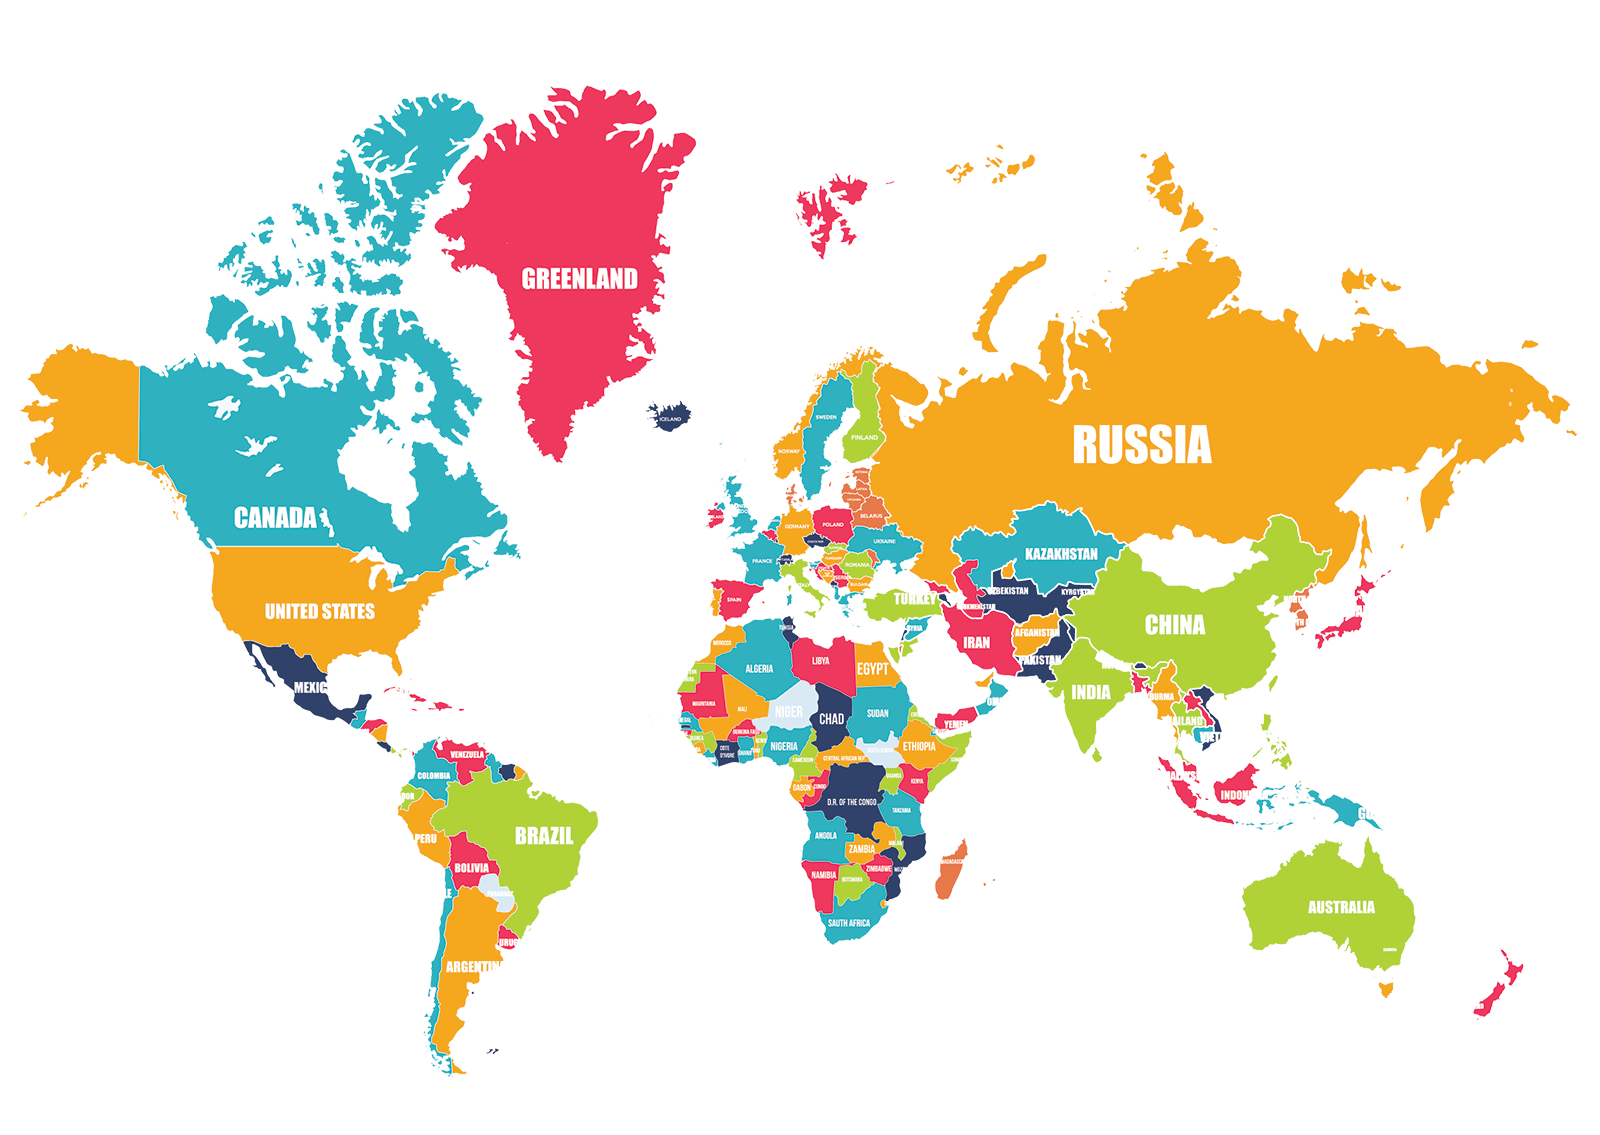
\includegraphics[width=\linewidth]{img/world-map}
			\caption{World map 3}
			\label{fig:world-map3}
		\end{figure}
		
	\end{multicols}

\end{frame}

\begin{frame}{Animated images}

Lorem ipsum dolor sit amet, consectetur adipiscing elit

\end{frame}

\section{Tables}
\begin{frame}{Add a table}

Lorem ipsum dolor sit amet, consectetur adipiscing elit

\end{frame}


\begin{frame}
	\centering\Huge\textcolor{orange}{\textbf{Thank you!}}
\end{frame}

\section{References}
\begin{frame}{References}
	\begin{tiny}\bibliography{bibliography}\end{tiny}
\end{frame}


\end{document}
